\section{Design}
\label{sec:design}

In this section, we describe the design of \ac{name}. We begin with an overview
of \ac{name}'s design. We then describe in detail the two main components of
\ac{name}:
\begin{inparaenum}[(1)]
\item a mechanism to signal which domains have deployed \ac{https}, and
\item a mechanism to enable the verification of multiple certificate chains.
\end{inparaenum}
We conclude the section with a description of how these components enable the
bootstrapping of more advanced policies \steve{cite ARPKI, etc.\@ here?}

\subsection{Overview}
\label{sec:design:overview}

\begin{figure}
  \centering 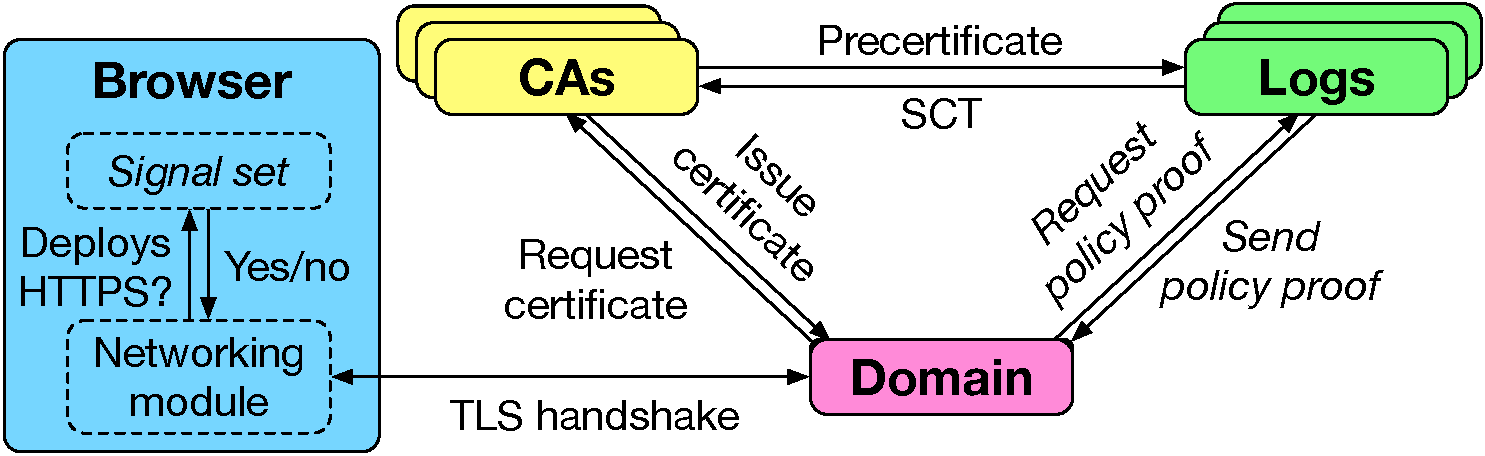
\includegraphics[width=\linewidth]{fig/overview} \caption{Overview
    of \ac{name} architecture (log auditors and monitors not shown). The browser
    is part of the client. Dotted lines denote browser components, and italic
  text denotes new components or actions in \ac{name}. \steve{TODO: update}}
  \label{fig:overview}
\end{figure}

\ac{name} aims to provide mechanisms for smoothly transitioning the current
\ac{pki} during the deployment of a \ac{pki} improvement or a new \ac{pki}
(hereafter simply referred to as the improved \ac{pki}). During this deployment
process, \ac{name} must
\begin{inparaenum}[(1)]
\item ensure that clients and domains that support the improved \ac{pki} use
  this \ac{pki} to negotiate encrypted connections, and
\item public keys in the improved \ac{pki} can be protected against concerted
  misbehavior by $n$ \acp{ca}, where each domain can choose a desired
  nonnegative value of $n$.
\end{inparaenum}

\autoref{fig:overview} illustrates the \ac{name} architecture and the steps by
which \ac{name} achieves the goals stated above. Since \ac{name} seeks to
transition from the current Web \ac{pki}, it necessarily includes the entities
present in the current \ac{pki}:
\begin{compactitem}
\item \emph{Domains} serve webpages to clients. Each domain has a name such as
  \texttt{example.com}.
  \steve{Put somewhere the rules of how domain names are
  differentiated, like www.example.com being a distinct name}
\item \emph{\acp{ca}} issue certificates to domains. Each certificate binds a
  set of names to a single public key.
\item \emph{Clients} connect to domains over HTTP or \ac{https}, and in the
  latter case, verify the binding between a domain's name and public key.
\item \emph{Browser/OS vendors} (hereafter simply \emph{vendors}) provide the
  software by which clients connect to domains and verify domains' certificates.
  \steve{Vendors also name a set of root \ac{ca} keys.}
\item \emph{Public logs} maintain a publicly auditable, append-only database of
  certificates.
\end{compactitem}
\ac{name} introduces two new entities:
\begin{compactitem}
\item The \emph{signaling authority} uses data from public logs to construct a
  set of all domains that have deployed \ac{https}.
\item The \emph{log aggregator} uses data from public logs to maintain the
  information that clients use to determine a domain's public key in the
  improved \ac{pki}.
\end{compactitem}
We present the signaling authority and log aggregator as independent entities,
but in \autoref{sec:discussion} we argue why browser vendors and public logs in
the current Web \ac{pki} should respectively take on the responsibilities of
these two entities.

In \ac{name}, the signaling authority constructs a \emph{signaling set}, which
represents the set of all domains that deploy HTTPS. To minimize the storage and
memory overhead of the signaling set, we represent the set as a
\emph{\ac{dafsa}} and apply data compression techniques to this representation.
\steve{When the final set of compression techniques is decided, briefly
summarize them here.} Clients download the signaling set and updates from the
signaling authority and use this set when connecting to domains to determine
whether to expect to connect over HTTP or HTTPS.

\ac{name} uses a simple, intuitive policy to determine a domain's public key in
the improved \ac{pki}: \emph{treat whichever public key is backed by the most
independent certificate chains as authoritative in the improved \ac{pki}}. By
\emph{independent} we mean that the certificate chains share no public keys
except at the leaf. Our policy also implies that if $n$ is the highest number of
observed independent certificate chains for a given domain, then \emph{any}
public key backed by $n$ chains can be used as that domain's in the improved
\ac{pki}. Thus, it is possible for a domain to have multiple public keys in the
improved \ac{pki}.\endnote{In practice, any improved \ac{pki} can enforce the
  use of a single public key by, for example, considering the first key backed
by $n$ chains as authoritative and using a ``cool-off period'' as in
AKI~\cite{kim2013accountable}.}

To implement this policy, the log aggregator pulls data from public logs to
create a complete view of all certificates in the Web \ac{pki}. From this, the
log aggregator extracts the set of all currently valid certificates, and uses
the certificate chains and leaf keys to create a mapping of domain names to
policies. To implement the policy we describe above, it is sufficient for the
log aggregator to simply map each domain name to the highest number of currently
valid independent certificate chains for that domain.

%To move towards \iac{pki} with increased resilience to the compromise of trusted
%parties (i.e., \acp{ca}), we need to prevent \iac{ca} that misissues a
%certificate for a domain from exposing that domain to \iac{mitm} attack. We
%observe that signatures from multiple independent \acp{ca} on a single public
%key can spur greater trust in the key, and therefore we design \ac{name} around
%the idea that domains should be able to obtain and communicate the presence of
%multiple certificates for a single public key. We can then protect domains from
%\ac{mitm} attacks by simply communicating to the client the number of
%certificates to expect. This approach results in simple policies that require
%domain involvement only in rare cases of deliberate misissuance, and allow
%security-conscious domains to ``ratchet up'' their security to their desired
%level.

%\ac{name} leverages \ac{ct}'s infrastructure in its policy mechanism, and
%therefore the two systems have similar architectures, as shown in
%\autoref{fig:overview}. \steve{TODO: add Censys data and an external service or
%browser vendor to the overview figure} \ac{name} assumes a full deployment of
%\ac{ct}, that is, all certificates must be logged for clients to accept them as
%valid. \steve{Beginning in October 2017, Chrome will begin enforcing this
  %requirement for all \ac{https} sites, so this assumption is a reasonable one.}
  %For the purposes of obtaining \acp{sct}, the logging process works just as it
  %does in \ac{ct}. Also as with \ac{ct}, public logs are kept accountable by
  %auditors and monitors, and an external party (Google in the case of \ac{ct})
  %maintains a list of known trusted logs.

%In \ac{name}, however, logs maintain an additional database of certificate
%policies alongside their database of certificates. The logging process also
%triggers changes in this policy database. Domains periodically request the proof
%for their latest policy from the logs and provide both their policy and proof to
%clients during the \ac{tls} handshake. We further describe the details of our
%policy mechanism in \autoref{sec:policy}.

%Client browsers locally maintain a \emph{signal set}, which indicate whether or
%not a given domain has deployed \ac{https}. The browser queries the signal set
%before initiating an HTTP or \ac{https} connection to a site 
%in order to determine
%\begin{inparaenum}
%\item whether or not to establish \iac{https} connection, and
%\item if so, how many certificates to expect.
%\end{inparaenum}
%If the signal set indicates that the domain has deployed \ac{https} but the
%server does not provide a certificate, the browser aborts the connection,
%assuming that an adversary is attempting to mount \iac{tls} stripping attack.

%The signal set is created by using data from the \ac{ct} logs. This data is used
%to construct a list of all DNS names for which a \ac{tls} certificate has been
%observed (either as the main subject or as a subject alternative name). This
%list is then represented using \iac{dafsa} that recognizes the DNS names of
%sites that deploy \ac{https}. By using compression techniques, we compact this
%\ac{dafsa} into a representation that requires little storage. Such a compact
%representation allows us to store the \ac{dafsa} in memory, offering performant
%lookups. We further describe the details of our signal set design in
%\autoref{sec:design:signaling}.

\subsection{Signaling HTTPS Deployment}
\label{sec:design:signaling}

\subsection{Verifying Multiple Certificate Chains}
\label{sec:design:verifying}

\subsection{Bootstrapping Advanced Policies}
\label{sec:design:bootstrapping}

